\documentclass[11pt]{article}

\usepackage{graphicx}
\pagestyle{myheadings}
\oddsidemargin=-0.3cm
\evensidemargin=-0.3cm
\textwidth=16.7cm
\topmargin=-0.8cm
\textheight=23.5cm
\renewcommand{\topfraction}{0.99}
\frenchspacing
\sloppy

%\renewcommand{\baselinestretch}{1.1}


\begin{document}

\setlength{\baselineskip}{25pt}


\begin{center}
{\huge \bf {Grid refinement in ICON: \\ technical description}} \\ \bigskip
{\Large G\"unter Z\"angl, DWD}
\end{center}

\setlength{\baselineskip}{14pt}

\bigskip

\section{Parent-child index relationships}

Parent-child index relationships describing the connectivity of grid points at different nesting levels
exist for cells and edges. They are provided by the grid generator.
The related fields in the \verb+t_patch+ data type are named \verb+child_idx+, 
\verb+child_blk+, \verb+parent_idx+ and \verb+parent_blk+. 
The parent index/block fields always carry nonzero values except for halo points related to the MPI domain
decomposition. In the global domain, the parent indices point to the next coarser grid level of the grid
generation hierarchy, which can be useful for hierarchical searching algorithms. Moreover, there is an
option to use the next coarser global grid level for computationally expensive physics parameterizations
(most prominently, radiation). The child index/block fields carry nonzero
values for all cells overlapping with a nested domain. As the refinement ratio between successive nesting
levels is fixed to a value of 2 (in terms of mesh size), each parent cell has four child cells. 
For edges, the child index/block fields also carry four values per parent edge. The first two indices
refer to the child edges aligned with the parent edge, whereas the child edge indices 3 and 4 refer
to the edges of the inner child cells that have (approximately) the same orientation as the parent cell.
For edges constituting the outer boundary of a nested domain, only three child edges exist (i.e. have a nonzero value).

An additional index field is available to cope with the fact that a model domain is allowed to have more 
than one child domain at the same nesting level. For cells and edges, a field named \verb+child_id+ indicates
the domain ID of the nested domain to which the child points of the current grid point belong. Note in this
context that a domain ID of 1 always denotes the global domain except when using the limited-area mode.


\section{Flow control mechanisms}

The flow control related to the grid refinement capability is primarily based on
\begin{itemize}
\item
patch fields indicating the distance from a lateral domain boundary, or from the lateral boundary of a nest overlap region,
\item
and a related reordering of the grid points that avoids IF-clauses during runtime.
\end{itemize}


\begin{figure*}[t!]
\vspace{-2cm}

\centering

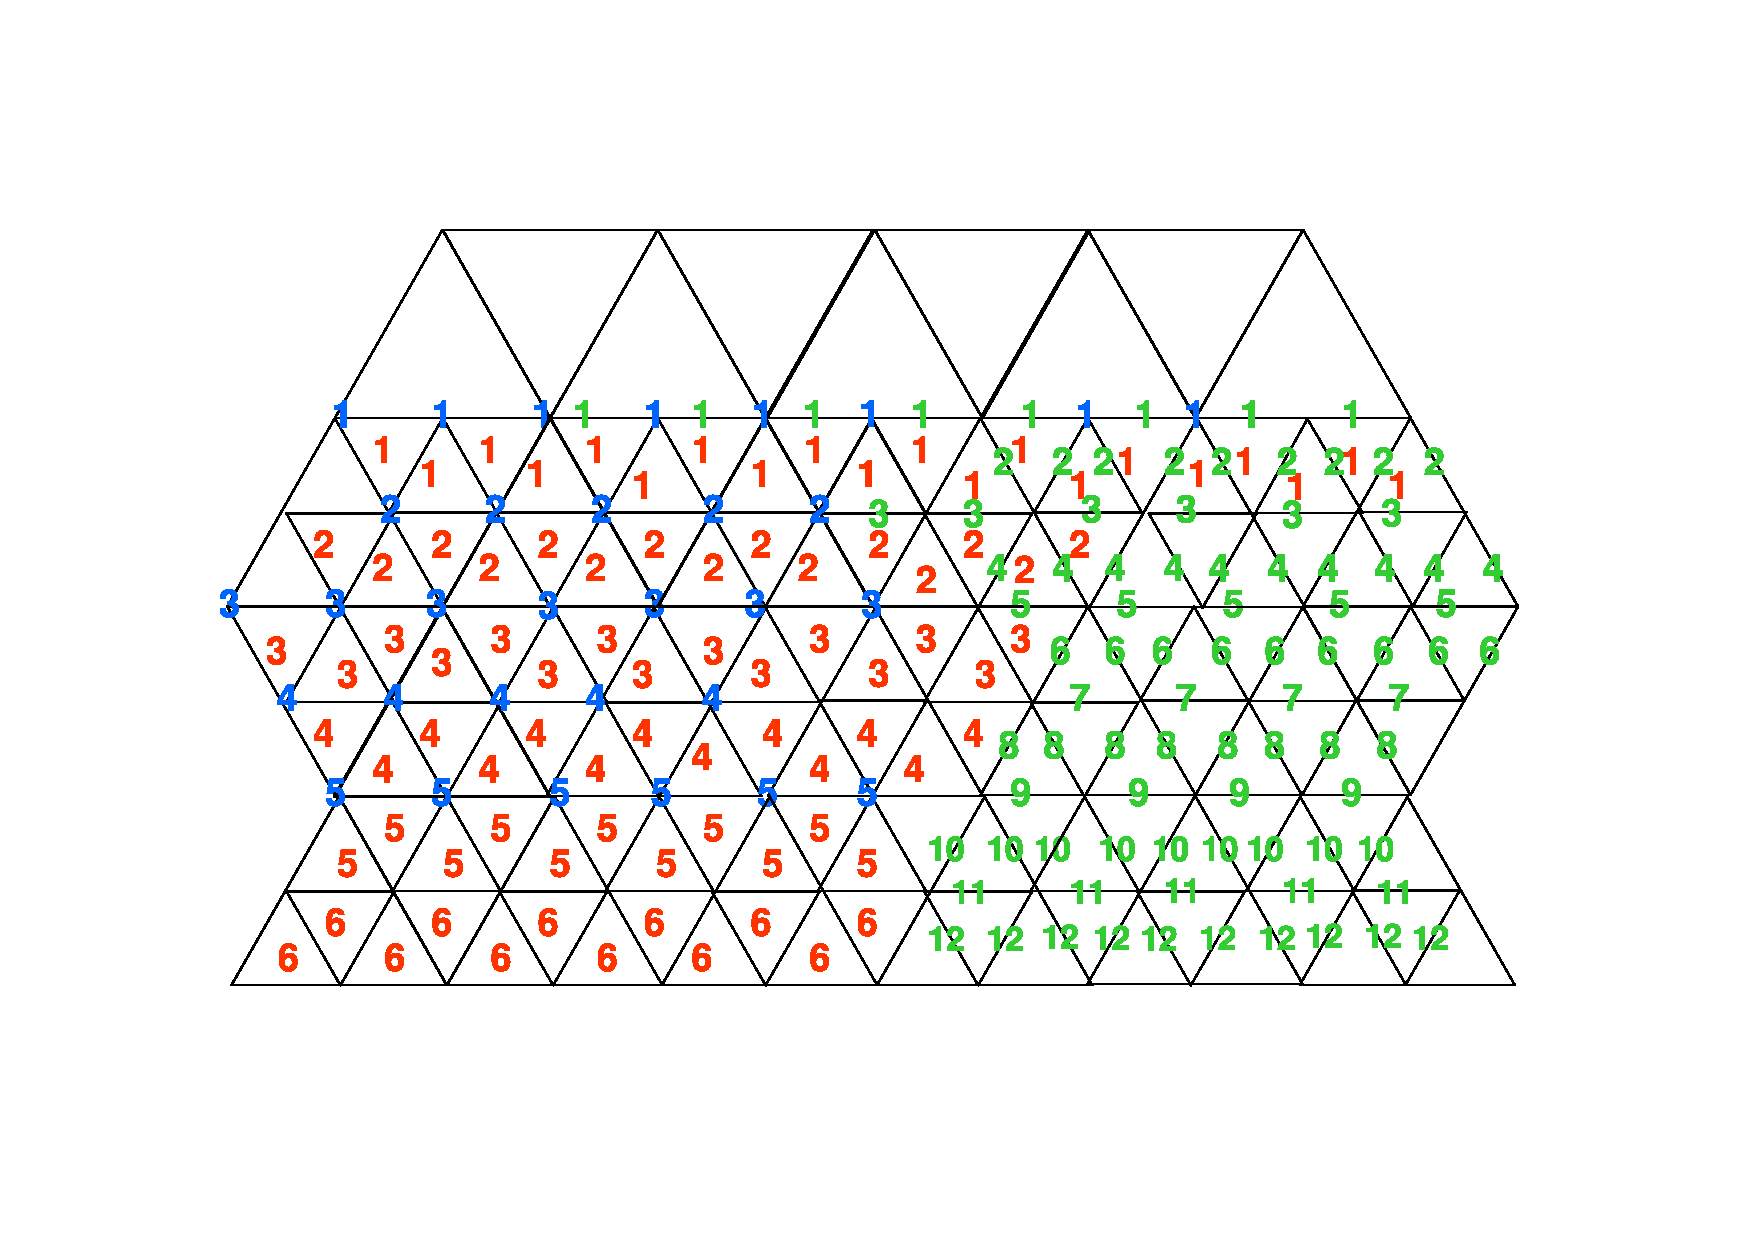
\includegraphics[width=\textwidth]{./icondoc_fig1}
\vspace{-2cm}

 \caption{Schematic view of the flagging of cells (red), edges (green) and vertices (blue) along the
lateral boundary of a nested domain.
}  

\end{figure*}

\subsection{Flag fields}

The above-mentioned flag fields are named \verb+refin_ctrl+ and exist for cells, edges and vertices. 
They are provided by the grid generator. For global grids not having any nested domains, the \verb+refin_ctrl+ flag
is zero everywhere. 

Along the lateral boundary of a nested domain, the \verb+refin_ctrl+ flags carry positive values (see Fig. 1). For cells, they
indicate the shortest distance to the boundary in units of cell rows. A similar counting is applied for vertices,
values of 1 indicating vertices lying along the outer boundary of a nested domain. For edges, however, the counting
proceeds twice as fast, with values of 1 indicating outer boundary edges, 2 indicating edges between cells of row 1, 
3 indicating interface edges between cell rows 1 and 2, etc. The reason for this finer granulation lies in the fact that
edge-based operations frequently involve only the adjacent cells; for example, a horizontal gradient can already be 
computed for edges flagged with 2, connecting cells of row 1. The number of cell rows flagged with a positive 
\verb+refin_ctrl+ value is specified by the namelist parameter \verb+bdy_indexing_depth+ in namelist \verb+gridref_ini+.
The default value of this parameter is 12, it must not be less than 10. Flagging of edges and vertices stops at
the interface between the last and the last-but-one cell row.

Negative \verb+refin_ctrl+ flags indicate grid points overlapping with a nested domain. i.e. all grid points
having child cells (or child edges) carry negative flags (see Fig. 2). Flagging starts with -1 along the outer
boundary of a nested domain, and counting towards the interior of the nest overlap region proceeds basically in the
same way as for lateral boundary cells, except that the descending flagging extends over a narrower zone
than the ascending flagging of boundary cells. Specifically, the three outer cell rows of the nest overlap
region have consecutively descending flags, whereas all remaining overlap points are flagged with a value of $-4$
for cells and vertices, and $-8$ for edges. In the model code, the corresponding parameters are named
\verb+min_rlcell_int+, \verb+min_rledge_int+ and \verb+min_rlvert_int+, respectively, and defined in 
\verb+mo_impl_constants+.

\begin{figure*}[t!]
\vspace{-2cm}

\centering

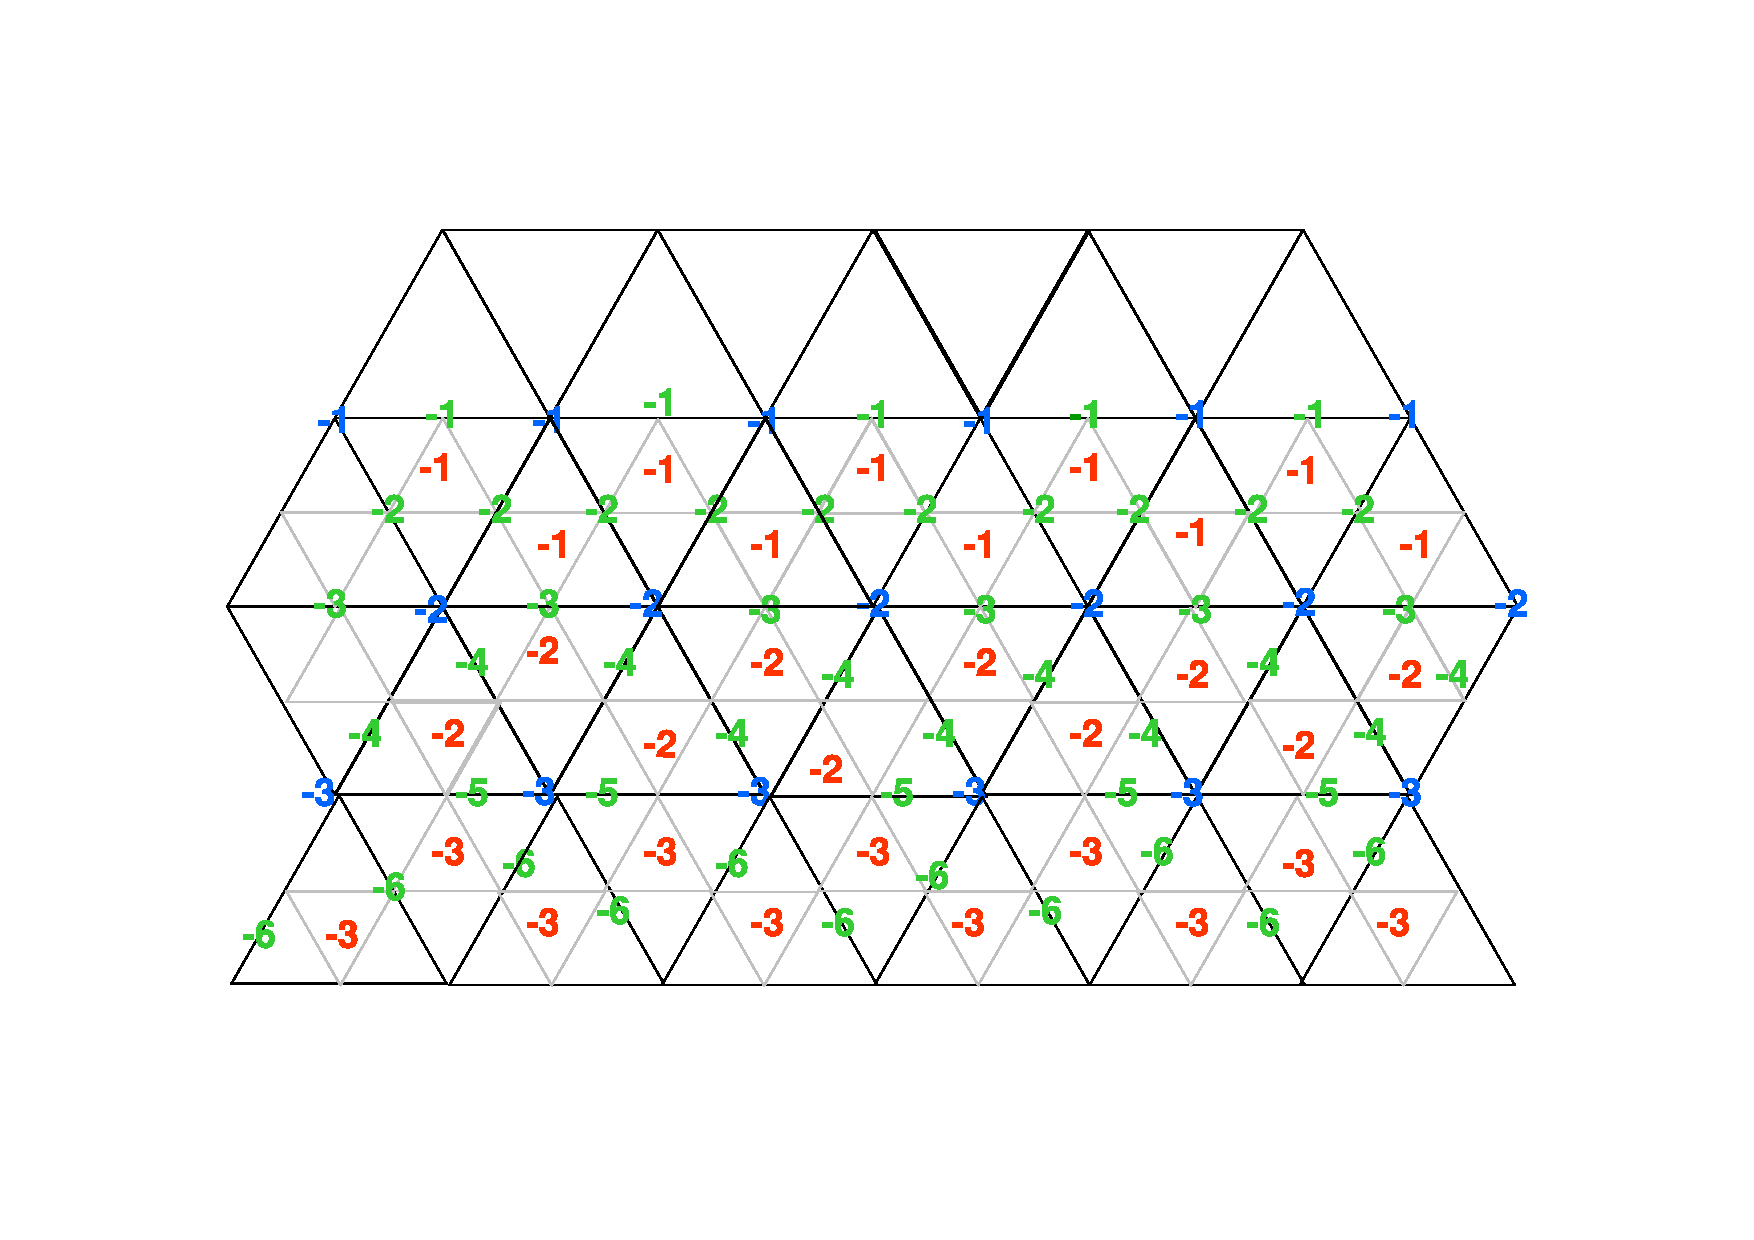
\includegraphics[width=\textwidth]{./icondoc_fig2}

\vspace{-2cm}

 \caption{Schematic view of the flagging of cells (red), edges (green) and vertices (blue) in the
overlap region of a nested domain (seen from the parent domain).
}  
\end{figure*}

\subsection{Grid point ordering}

To achieve computationally efficient runtime flow control without the need of setting IF-clauses inside
do loops, the model grid points are ordered according to their \verb+refin_ctrl+ flag. Lateral boundary
points (if present) come at the beginning of the index list, followed by interior grid points not overlapping
with a nested domain (i.e. having a \verb+refin_ctrl+ flag of 0). Grid points overlapping with a nested domain
come at the end of the index list. In the presence of an MPI domain decomposition, the related halo points
come at the very end of the index list. This implies that for horizonal stencil operations involving grid points
that are not available along the lateral boundary of a nested domain, the related DO loop simply starts in
a grid cell row where the required neighbor points are available. Likewise, DO loops executing parent-to-child 
interpolation operations start at the index that corresponds to the beginning of the nest overlap zone.


The code parameters governing the depth of the index ordering are defined in \verb+mo_impl_constants+.
The number of grid cell rows, and related edges and vertices, that is shifted at the beginning of the 
index list is given by \verb+max_rlcell+, \verb+max_rledge+ and \verb+max_rlvert+, respectively.
These parameters are currently set to 5, 10 and 5, respectively, which implies that the number of
ordered boundary rows is less than the number of flagged boundary rows (see above). These values correspond
to the beginning of the part of nested domains for which the model equations are solved prognostically
(as opposed to the boundary interpolation zone). The wider zone with \verb+refin_ctrl+ flags is needed only
for some special operations like for instance the nudging required in the case of one-way nesting. 
For grid points overlapping with a nested domain, the ordering follows exactly the \verb+refin_ctrl+ flags
as described above. 

The index lists carrying the related start and end indices for each segment are defined in the \verb+t_patch+ data type
and exist for cells, edges and vertices. They are named \verb+start_idx+ / \verb+start_blk+ and \verb+end_idx+ / 
\verb+end_blk+ and have two dimensions, the first one going from \verb+min_rlcell+ to \verb+max_rlcell+ for cells, 
from \verb+min_rledge+ to \verb+max_rledge+ for edges and from \verb+min_rlvert+ to \verb+max_rlvert+ for vertices, 
and the second one being the highest number of child domains per parent domain (as inferred from the namelist settings 
specified by the user). Note that the child domain counter matters only for the nest overlap region, i.e. the list
segments described by a negative first index. The index range between \verb+min_rl*+ and \verb+min_rl*_int - 1+ is
reserved for MPI halo points (see below).

As already indicated, the list segments \verb+(1:max_rl*,:)+ refer to the
lateral boundary rows of nested domains. For global domains, they are empty, i.e. \\
\verb+    start_idx(1:max_rl*,:) = 1+ and \\
\verb+    end_idx(1:max_rl*,:)   = 0+ (and the related block values are always 1). \\
For global domains having no nests, \verb+start_idx(0,:) = 1+, \verb+start_blk(0,:) = 1+, and \verb+end_idx(0,:)+ /
\verb+end_blk(0,:)+ carry the last prognostic (non-halo) model grid point.
Otherwise, the nest overlap region starts at \verb+(start_blk(-1,1), start_idx(-1,1))+, and 
\verb+(end_blk(min_rl*_int,1),+ \verb+end_idx(min_rl*_int,1))+ denotes the end of the overlap region with the first
nested domain. If there is another nested domain, the related overlap region comes after the end of the first one.
In the presence of an MPI domain decomposition, the related halo points come after the end of the
last nest overlap zone. The halo zone starts at \verb+(start_blk(min_rl*_int-1,1),start_idx(min_rl*_int,1))+
and ends at \verb+(end_blk(min_rl*,1),end_idx(min_rl*,1))+. Without MPI parallelization, these index segments
are empty.


\subsection{More flow control parameters}

A number of further parameters needed for runtime flow control are defined in \verb+mo_impl_constants_grf+.
\begin{itemize}
\item
\verb+grf_bdywidth_c = 4+ and \\
\verb+grf_bdywidth_e = 9+ \\
denote the width of the lateral boundary interpolation zone
of nested domains. On the grid points lying in these boundary rows, the prognostic variables are interpolated
from the parent domain, rather than being computed prognostically.
\item
\verb+grf_bdyintp_start_c = -1+,\\
\verb+grf_bdyintp_start_e = -1+,\\
\verb+grf_bdyintp_end_c   = - grf_bdywidth_c/2+ and\\
\verb&grf_bdyintp_end_e   = -(grf_bdywidth_e+1)/2&\\
denote the corresponding grid points at parent level, on which the interpolation to the above-mentioned
child points is executed.
\item
\verb+grf_ovlparea_start_c = -1+\\
denotes the start of the nest overlap area. This parameter could be regarded as redundant, but at some
places in the code where no interpolation is performed, it was felt that a parameter with this name
is more appropriate.
\item
\verb+grf_fbk_start_c = -3+ and\\
\verb+grf_fbk_start_e = -5+\\
denote the start of the feedback area for cell- and edge-based variables. Note that the feedback domain
for edge-based variables (velocity) overlaps with the boundary interpolation zone by one edge row (for
numerical reasons), whereas there is no overlap for cell-based variables.
\item
\verb+grf_nudgezone_width = 8+\\
denotes the width of the boundary nudging zone needed in case of one-way nesting. This parameter may
be sufject to changes because boundary nudging still requires some tuning.
\item
\verb&grf_nudge_start_c = grf_bdywidth_c + 1&, \\
\verb&grf_nudge_start_e = grf_bdywidth_e + 1&, \\
\verb&grf_nudge_end_c   = grf_nudge_start_c + grf_nudgezone_width& and \\
\verb&grf_nudge_end_e   = grf_nudge_start_e + grf_nudgezone_width*2& \\
indicate the extent of the boundary nudging zone as seen from the child domain.
\item
\verb&grf_nudgintp_start_c = grf_bdyintp_end_c - 1&,\\
\verb&grf_nudgintp_start_e = grf_bdyintp_end_e&, \\
\verb&grf_nudgintp_end_c   = - grf_nudge_end_c/2& and \\
\verb&grf_nudgintp_end_e   = -(grf_nudge_end_e+1)/2& \\
indicate the extent of the boundary nudging zone as seen from the parent domain, i.e. the 
cells/edges on which parent-to-child interpolation needs to be performed.
\end{itemize}



\section{Organization of MPI halo points}

The organisation of the MPI halo points is based on another set of internal flags that are, however,
only temporarily available in \verb+mo_subdivision+. The most important difference to the flagging
of nest boundary points is that the ordering of halo cells has a finer granulation in order to
optimally exploit the potential for optimization. The present implementation, in particular the
space reserved in the \verb+start_idx/blk+ and \verb+end_idx/blk+ fields, is set up for a maximum
halo width (\verb+n_ghost_rows+ in namelist \verb+parallel_ctl+) of 2 full cell rows. While
it is unlikely that \verb+n_ghost_rows = 2+ will be used in operational application, there may
appear higher-order methods that require this halo width. 

The ordering of the halo points is as follows:\\
\verb+min_rlcell_int - 1+: halo cells having a prognostic cell as neighbor \\
\verb+min_rlcell_int - 2+: halo cells in the first cell row having no prognostic cell as neighbor \\
and analogously for the second halo cell row if present. For \verb+n_ghost_rows = 1+, the index segments
corresponding to \verb+min_rlcell_int - 3+ and \verb+min_rlcell_int - 4+ (= \verb+min_rlcell+) are empty.

For edges and vertices, one needs to be aware of the fact that outer boundary edges/vertices of a prognostic
cell may not be owned by the current PE because the PE of the neighboring cell has the ownership (otherwise
there would be double-counting). There are, however, operations for which even such edges/vertices can be 
excluded from prognostic computation because a halo synchronization follows immediately afterwards (and
has to be there anyway). Thus, the following ordering is applied: \\
\verb+min_rledge_int - 1+: outer boundary edges of a prognostic cell not owned by the current PE\\
\verb+min_rledge_int - 2+: edges connecting halo cells of the first row\\
\verb+min_rledge_int - 3+: outer boundary edges of the first halo cells row, or edges connecting cells
of the first halo cell row with cells of the second halo cell row.\\
For \verb+n_ghost_rows = 2+, an analogous setting applies to \verb+min_rledge_int - 4+ and 
\verb+min_rledge_int - 5+ (= \verb+min_rledge+). For vertices, we have\\
\verb+min_rlvert_int - 1+: outer boundary vertices of a prognostic cell not owned by the current PE\\
\verb+min_rlvert_int - 2+: outer boundary vertices of the first halo cells row, or vertices connecting cells
of the first halo cell row with cells of the second halo cell row.\\
For \verb+n_ghost_rows = 2+, an analogous setting applies to \verb+min_rlvert_int - 3+ 
(= \verb+min_rlvert+).


\end{document}
